\chapter{Ćwiczenie 2 - czwórnik CR}

\section{Polecenie}

Należało sprawdzić odpowiedź układu różniczkującego (\textbf{CR}) na podawaną na wejście falę prostokątną o zadanym okresie \textbf{T}. \\ 
Następnie zaobserwować odpowiedź układu na impuls trójkątny. 

\section{Odpowiedź na falę prostokątną}

Wybrano okres \textbf{T} równy:
\begin{enumerate}
    \label{poprawa:dodanie_wartosci_tau_3_2}
    \item \textbf{T = 0.1}$\boldsymbol{\tau}$ = \textbf{125Hz}
    \item \textbf{T = 1}$\boldsymbol{\tau}$ = \textbf{1.25kHz}
    \item \textbf{T = 10}$\boldsymbol{\tau}$ = \textbf{12.5kHz}
\end{enumerate}

\begin{figure}[H]
    \centering
    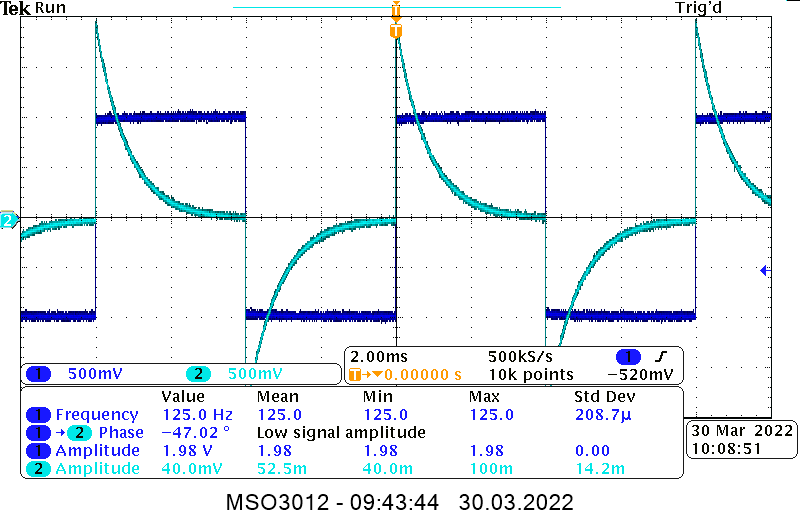
\includegraphics[scale=0.25]{img_osciloscope/CR_pros_troj/CR_prostokatna_mniejsze_tau_cropped.png}
    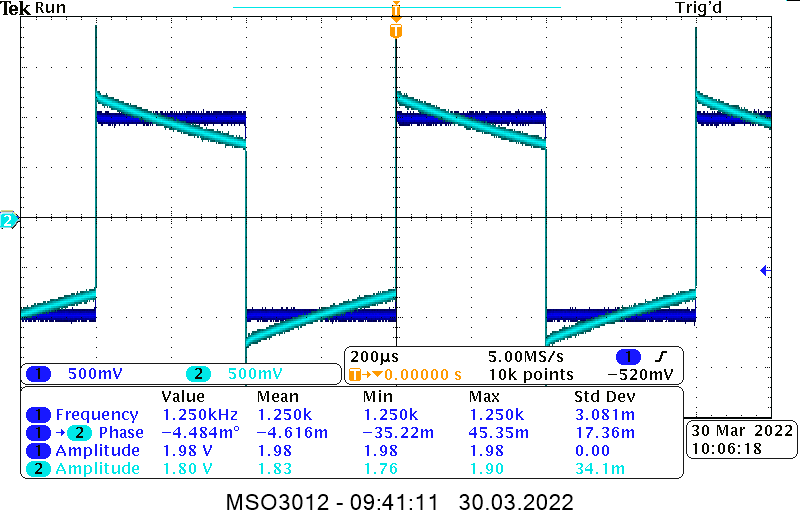
\includegraphics[scale=0.25]{img_osciloscope/CR_pros_troj/CR_prostokatna_rowne_tau_cropped.png}
    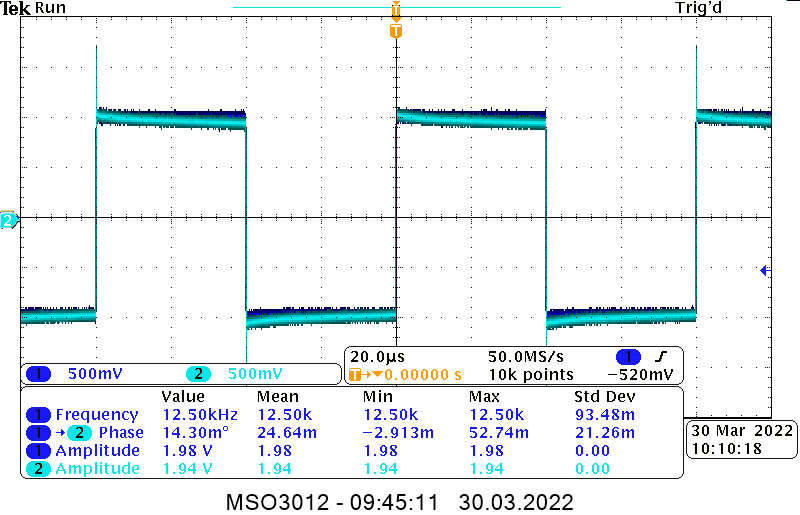
\includegraphics[scale=0.25]{img_osciloscope/CR_pros_troj/CR_prostokatna_wieksze_tau_cropped.png}
    \label{fig:CR_trojkatna}
\end{figure}

Sygnał wyjściowy zgadza się z teoretycznym, układ poprawnie różniczkuje sygnał prostokątny.

\begin{figure}[H]
    \centering
    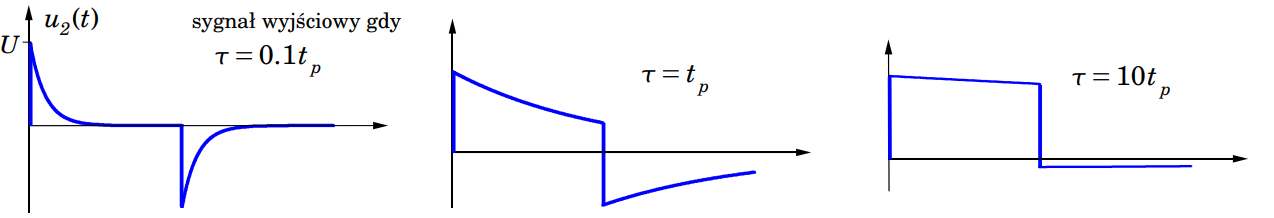
\includegraphics[width=\textwidth]{img_wyklad/teor_pros_CR.png}
    \caption{Teoretyczne wykresy prostokątnych sygnałów przechodzących przez układ CR}
    \label{fig:my_label}
\end{figure}

\newpage

\section{Odpowiedź na falę trójkątną}

Wybrano okres \textbf{T} rowny:
\begin{enumerate}
    \label{poprawa:dodanie_wartosci_tau_3_3}
    \item \textbf{T = 0.1}$\boldsymbol{\tau}$ = \textbf{125Hz}
    \item \textbf{T = 1}$\boldsymbol{\tau}$ = \textbf{1.25kHz}
    \item \textbf{T = 10}$\boldsymbol{\tau}$ = \textbf{12.5kHz}
\end{enumerate}

\begin{figure}[H]
    \centering
    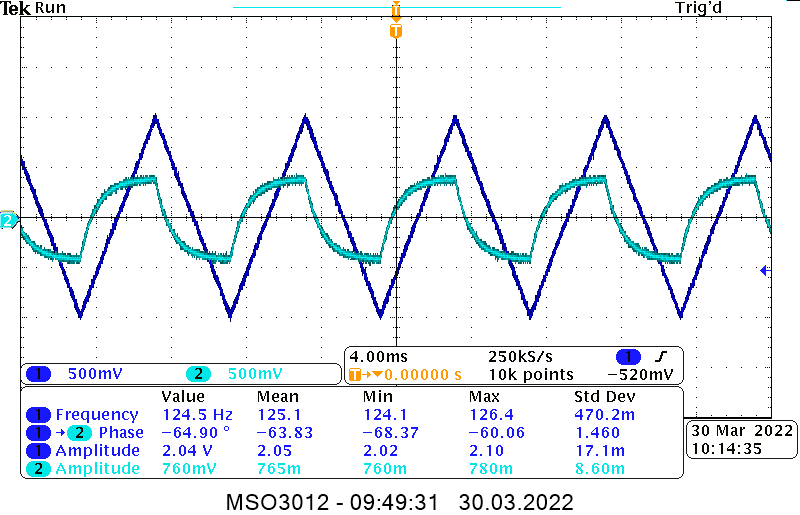
\includegraphics[scale=0.25]{img_osciloscope/CR_pros_troj/CR_trojkatna_mniejsze_tau_cropped.png}
    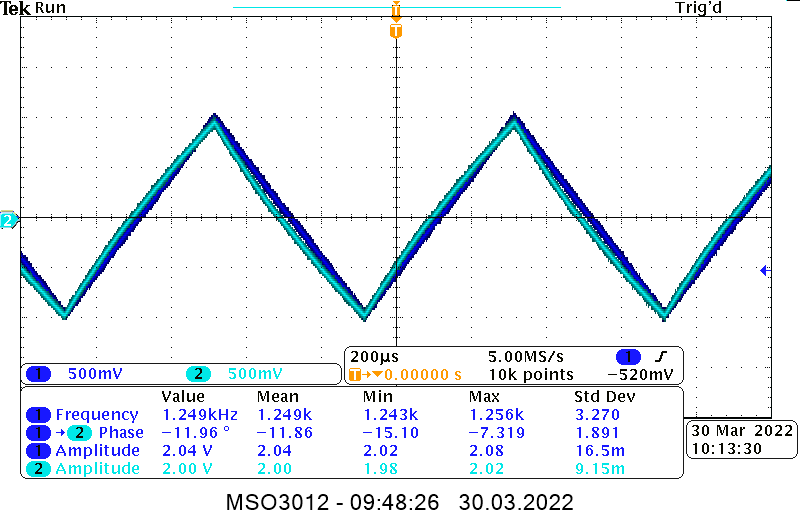
\includegraphics[scale=0.25]{img_osciloscope/CR_pros_troj/CR_trojkatna_rowne_tau_cropped.png}
    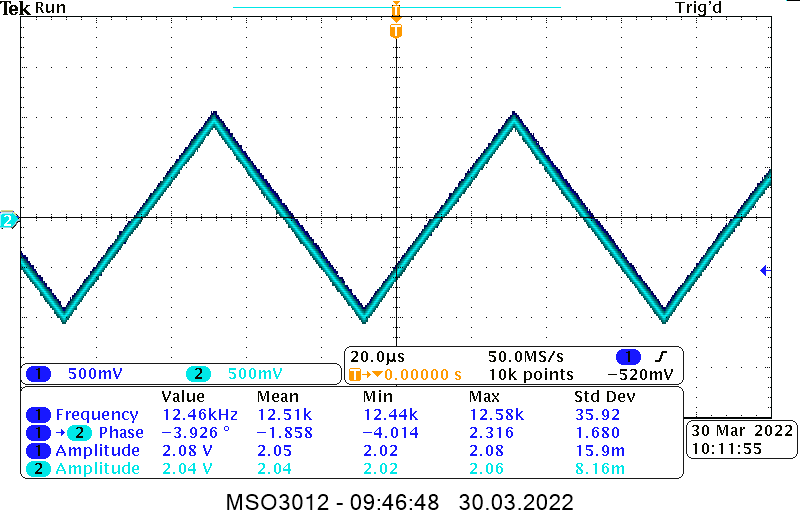
\includegraphics[scale=0.25]{img_osciloscope/CR_pros_troj/CR_trojkatna_wieksze_tau_cropped.png}
    \label{fig:CR_trojkatna}
\end{figure}

Sygnał wyjściowy zgadza się z teoretycznym, układ poprawnie różniczkuje sygnał trójkątny.